\section{Технологический раздел}\label{sec:technic}
\subsection{Использование компилятора}\label{subsec:compilation}
Рассмотрим работу компилятора на примере компиляции программы сортировки массива целых чисел на языке Golang.
Исходный код представлен в листинге~\ref{lst:src}
\begingroup
\lstinputlisting[language=go,caption={Исходный код на языке Golang},label={lst:src}]{code/main.go}
\endgroup

Абстрактное синтаксическое дерево для данной программы слишком большое, поэтому на рисунке~\ref{fig:tree}
представлен пример AST для более простой программы, выводящей в стандартный поток вывода числа от 0 до 10.
\begin{figure}[h!]
    \centering
    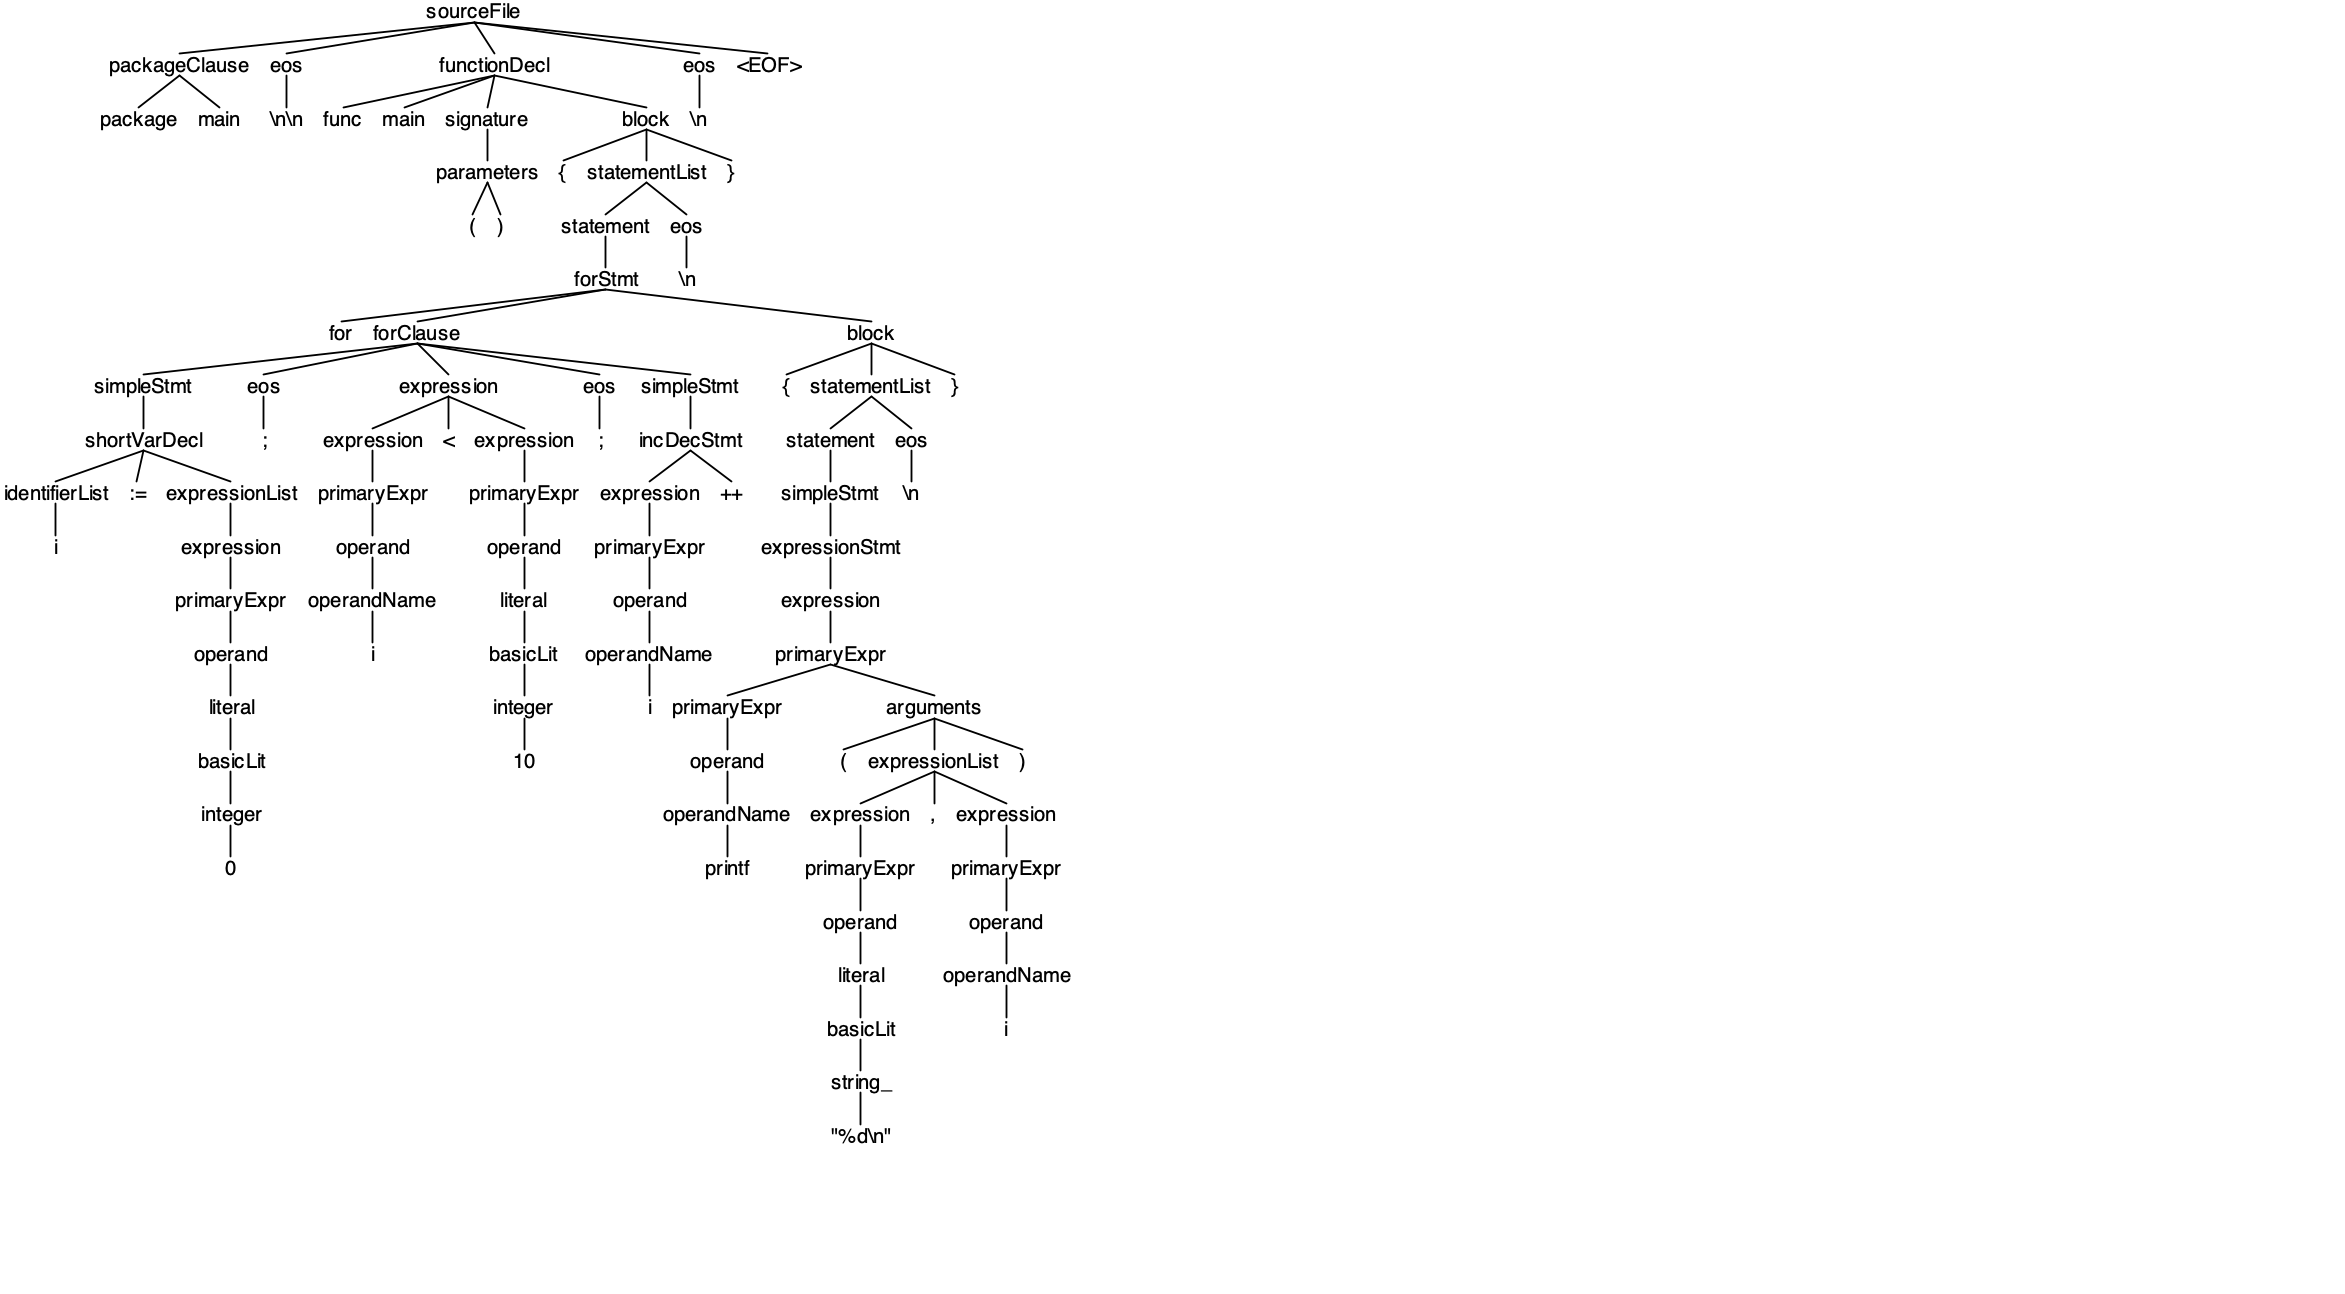
\includegraphics[scale=0.4]{img/tree}
    \caption{AST программы печати чисел от 0 до 10}
    \label{fig:tree}
\end{figure}

Результатом работы компилятора является код на языке промежуточного представляения LLVM IR, он представлен в
листинге~\ref{lst:ir}.
\begingroup
\lstinputlisting[language=llvm,caption={Код промежуточного предствления LLVM IR},label={lst:ir}]{code/main.ll}
\endgroup

